% -----------------------------------------------
% Template for ISMIR Papers
% 2016 version, based on previous ISMIR templates

% Requirements :
% * 6+1 page length maximum
% * 2MB maximum file size
% * Copyright note must appear in the bottom left corner of first page
% (see conference website for additional details)
% -----------------------------------------------

\documentclass{article}
\usepackage{ismir,amsmath,cite}
\usepackage{graphicx}
\usepackage{color}
\usepackage{amsfonts}

% Title.
% ------3
\title{Tempo Estimation for Music Loops and a Simple Confidence Measure}

% Note: Please do NOT use \thanks or a \footnote in any of the author markup

% Single address
% To use with only one author or several with the same address
% ---------------
\oneauthor
 {Frederic Font and Xavier Serra}
 {Music Technology Group, Universitat Pompeu Fabra \\ {\tt frederic.font@upf.edu}, {\tt xavier.serra@upf.edu}}

% Two addresses
% --------------
%\twoauthors
%  {Frederic Font} {School \\ Department}
%  {Xavier Serra} {Company \\ Address}

%% To make customize author list in Creative Common license, uncomment and customize the next line
%  \def\authorname{First Author, Second Author} 


% Three addresses
% --------------
%\threeauthors
%  {First Author} {Affiliation1 \\ {\tt author1@ismir.edu}}
%  {Second Author} {\bf Retain these fake authors in\\\bf submission to preserve the formatting}
%  {Third Author} {Affiliation3 \\ {\tt author3@ismir.edu}}

%% To make customize author list in Creative Common license, uncomment and customize the next line
%  \def\authorname{First Author, Second Author, Third Author} 

% Four or more addresses
% OR alternative format for large number of co-authors
% ------------
%\multauthor
%{First author$^1$ \hspace{1cm} Second author$^1$ \hspace{1cm} Third author$^2$} { \bfseries{Fourth author$^3$ \hspace{1cm} Fifth author$^2$ \hspace{1cm} Sixth author$^1$}\\
%  $^1$ Department of Computer Science, University , Country\\
%$^2$ International Laboratories, City, Country\\
%$^3$  Company, Address\\
%{\tt\small CorrespondenceAuthor@ismir.edu, PossibleOtherAuthor@ismir.edu}
%}
%\def\authorname{First author, Second author, Third author, Fourth author, Fifth author, Sixth author}


\sloppy % please retain sloppy command for improved formatting

\begin{document}

\maketitle

\begin{abstract}
Tempo estimation is a common task within the music information retrieval community, but existing works are rarely evaluated with datasets of music loops and the algorithms are not tailored to this particular type of content. In addition to this, existing works on tempo estimation do not put an emphasis on providing a confidence value that indicates how reliable their tempo estimations are. In current music creation contexts, it is common for users to search for and use loops shared in online repositories.
These loops are typically not produced by professionals and lack annotations. Hence, the existence of reliable tempo estimation algorithms becomes necessary to enhance the reusability of loops shared in such repositories. In this paper, we test six existing tempo estimation algorithms against four music loop datasets containing more than 35k loops. We also propose a simple and computationally cheap confidence measure that can be applied to any existing algorithm to estimate the reliability of their tempo predictions when applied to music loops. We analyse the accuracy of the algorithms in combination with our proposed confidence measure, and see that we can significantly improve the algorithms' performance when only considering music loops with high estimated confidence.
\end{abstract}

\section{Introduction}\label{sec:introduction}
Tempo estimation is a topic that has received considerable attention within the music information retrieval (MIR) community and has had a dedicated task in the Music Information Retrieval Evaluation eXchange (MIREX) since its first edition in 2005.
Tempo estimation consists in the automatic determination of the ``rate of musical beats in time''~\cite{Gouyon2006}, that is to say, in the identification of the rate at which periodicities occur in the audio signal that convey a rhythmic sensation.
Tempo is typically expressed in beats per minute (BPM), and is a fundamental property to characterise rhythm in music~\cite{Muller2015}. 
Applications of tempo estimation include, just to name a few, music recommendation, music remixing, music browsing, and beat-aware audio analysis and effects.

Our particular research is aimed at automatically annotating user provided music loops hosted in online sound sharing sites to enhance their potential reusability in music creation contexts.
We can define music loops as short music fragments which can be repeated seamlessly to produce an ``endless'' stream of music. 
In this context, BPM is an important music property to annotate.
The kind of music loops we are targeting can include noisy and low quality content, typically not created by professionals. 
This may increase the difficulty of the tempo estimation task. 
Taking that into consideration, it is particularly relevant for us to not only estimate the tempo of music loops, but to also quantify how reliable an estimation is (i.e.,~to provide a confidence measure). 
Except for the works described in~\cite{Gouyon2006,Oliveira2010} (see below), tempo estimation has been rarely evaluated with datasets of music loops, and we are not aware of specific works describing algorithms that are specifically tailored to this particular case.

In this paper we evaluate the accuracy of six state of the art tempo estimation algorithms when used to annotate four different music loop datasets, and propose a simple and computationally cheap confidence measure that can be used in combination with any of the existing methods. 
The confidence measure we propose makes the assumption that the audio signal has a steady tempo thorough its whole duration. 
While this assumption can be safely made in the case of music loops, it does not necessarily hold for other types of music content such as music pieces.
Hence, the applicability of the confidence measure we propose is restricted to music loops.
Using our confidence measure in combination with existing tempo estimation algorithms, we can automatically annotate big datasets of music loops and reach accuracies above 90\% when only considering content with high BPM estimation confidence. 
Such reliable annotations can allow music production systems to, for example, present relevant loops to users according to the BPM of a music composition, not only by showing loops with the same BPM but also by automatically transforming loops to match a target BPM. This effectively increases the reusability of user provided music loops in real-world music creation contexts. 

The rest of the paper is organised as follows. In Sec.~\ref{sec:related_work} we give a quick overview of related work about tempo estimation.
In Sec.~\ref{sec:confidence_measure} we describe the confidence measure that we propose. Sections~\ref{sec:evaluation_methodology} and~\ref{sec:results} describe the evaluation methodology and show the results of our work, respectively. We end this paper with some conclusions in Sec.~\ref{sec:conclusion}.
In the interest of research reproducibility, the source code and one of the datasets used in this paper have been made available online in a public source code repository\footnote{https://github.com/ffont/ismir2016}.
%This repository includes instructions on how to reproduce our results and extra plots and information.

\section{Related work}\label{sec:related_work}
A significant number of works within the MIR research field have been focused on the task of tempo estimation. 
%Some of the steps carried out by different algorithms are common and some others are distinctive of each algorithm.
In general, tempo estimation algorithms are based on detecting onsets in an audio signal, either as a continuous function~\cite{Davies2007a,Oliveira2010,Percival2014} or as discrete events in time~\cite{Dixon2001}. Then, a dominant period is extracted from the onsets either by analysing inter-onset intervals, using autocorrelation~\cite{Grosche2010} or resonating filters~\cite{Klapuri2006}. 
%This results in a number of tempo candidates and different heuristics can be used to decide in which is the most probable tempo. 
Some approaches perform more complex operations such as analysing periodicities in different frequency bands~\cite{Gainza2011,Wu2014}, performing source separation~\cite{Gkiokas2012,Elowsson2013}, or using neural networks to learn features to use instead of usual onset information~\cite{Sebastian2015}.

While comparative studies of tempo estimation algorithms have been carried out in the past~\cite{Gouyon2006,Zapata2011}, we are not aware of any study solely devoted to the evaluation of tempo estimation algorithms for music loops.
One of the typical datasets that some of the existing tempo estimation works use for evaluation is the ISMIR 2004 dataset released for the tempo induction contest of that year\footnote{http://mtg.upf.edu/ismir2004/contest/tempoContest}. This dataset is divided into three subsets, one of them composed of 2k audio loops. Gouyon et. al.~\cite{Gouyon2006} published the evaluation results for the contest considering the different subsets of the dataset, but no significant differences are reported regarding the accuracies of the tempo estimation algorithms with the loops subset compared to the other subsets. 
To the best of our knowledge, the only other work that uses the loops subset of the ISMIR 2004 dataset and reports its accuracy separated form other datasets is by Oliveira et. al.~\cite{Oliveira2010}. The authors report lower estimation accuracies when evaluating with the loops dataset and attribute this to the fact that loops are typically shorter than the other audio signals (in many cases shorter than 5 seconds).

Surprisingly enough, there has not been much research on confidence measures for tempo estimation algorithms.
Except for the work by Zapata et al.~\cite{Zapata2012} in which a confidence measure that can be used for tempo estimation is described (see below), we are not aware of other works directly targeted at this issue. 
Among these few, Grosche and M\"{u}ller~\cite{Grosche2010} describe a confidence measure for their tempo estimation algorithm based on the amplitude of a predominant local pulse curve. 
%The PLP curve represents periodicities in the signal by fitting sinusoidal kernels to the novelty curves of each analysis window and performing an overlap-add operation. Tempo inconsistencies in the signal produce destructive interferences in the PLP, resulting in peaks of less amplitude. The confidence is then defined by setting an amplitude threshold for the PLP curve and selecting regions whose corresponding PLP peaks are above that threshold. 
By analysing tempo estimation accuracy and disregarding the regions of the analysis with bad confidence, the overall accuracy significantly increases. 
Alternatively, Percival and Tzanetakis~\cite{Percival2014} suggest that beat strength~\cite{Tzanetakis2002} can be used to derive confidence for tempo candidates, but no further experiments are carried out to asses its impact on the accuracy of tempo estimation.
Finally, a very recent work by Quinton et. al.~\cite{Quinton2016} proposes the use of rhythmogram entropy as a measure of  reliability for a number of rhythm features, and report a statistical correlation between measured entropy and the resulting accuracies for different tasks.

\section{Confidence measure}\label{sec:confidence_measure}

\begin{figure*}
 \centerline{
 \includegraphics[width=0.95\textwidth]{figs/confidence_measure_examples-crop.pdf}}
 \caption{Visualisation of confidence computation output according to BPM estimation and signal duration (green curves). The top figure shows a loop whose annotated tempo is 140 BPM but the predicted tempo is 119 BPM.
	The duration of the signal $l^a$ does not closely match any multiple of $l^b$ (dashed vertical lines), and the output confidence is 0.59 (i.e.,~$1 - \frac{\Delta l}{\lambda}$).
 The figure at the bottom shows a loop that contains silence at the beginning and at the end, and for which tempo has been correctly estimated as being 91 BPM.
 The yellow curve represents its envelope and the vertical dashed red lines the estimated effective start and end points.
 Note that $l_2^a$ closely matches a multiple of $l^b$, resulting in a confidence of 0.97. The output confidence computed with $l^{a}$, $l_0^{a}$ and $l_1^{a}$ produces lower values.}
 \label{fig:confidence_measure_examples}
\end{figure*}

Assuming that we obtain a BPM estimate for a given audio signal, the confidence measure that we propose is based on comparing the duration of the whole audio signal with a multiple of the duration of a single beat according to the estimated BPM. If the actual duration of the signal is close to a multiple of the duration of a single beat, we hypothesise that the BPM estimation is reliable.
The first thing we do to compute the confidence measure is to round the estimated tempo value to its nearest integer.
The reasoning behind this is that it is very unlikely that loops are created with less than 1 BPM resolution tempo (see Sec.~\ref{sec:datasets}), and thus we consider the best BPM estimate of a tempo estimation algorithm to be its nearest integer.
Given the sample rate $SR$ of an audio signal and its estimated tempo $BPM^e$, we can estimate the duration (or length) of an individual beat in number of samples $l^b$ as
$$l^b = \frac{60 \cdot SR}{BPM^e}.$$ 
Then, potential durations for the audio signal can be computed as multiples of the individual beat duration, $L[n] = n \cdot l^b$, where $n \in \mathbb{Z}^+$.
In our computation, we restrict $n$ to the range $1 \le n \le 128$.
This is decided so that the range can include loops that last from only 1 beat to 128 beats, which would correspond to a maximum of 32 bars in 4/4 meter. 
In practice, what we need here is a number big enough such that we won't find loops longer than it.
Given $L$, what we need to see at this point is if any of its elements closely matches the actual length of the original audio signal. 
To do that, we take the actual length of the audio signal $l^a$ (in number of samples), compare it with all elements of $L$ and keep the minimum difference found:
%$$ \Delta l = min(|L - l^a|),$$
$$ \Delta l = \min\{|L[n]-l^a|:n\le 128\}. $$
%Note that $L$ is a vector and $l^a$ is a scalar, we therefore subtract $l^a$ to $L$ element-wise and take the absolute value. 
A value of $\Delta l$ near 0 means that there is a close match between one of the potential lengths and the actual length of the audio signal. 
Having computed $\Delta l$, we finally define our confidence measure as 
$$ 
confidence(L,l^a) = \begin{cases} 
	0 & \text{if } \Delta l > \lambda \\
    1 - \frac{\Delta l}{\lambda} & \text{otherwise}\\
\end{cases},
$$
where $\lambda$ is a parameter set to half the duration of a single beat ($\lambda = 0.5 \cdot l^b$). In this way, if $l^a$ exactly matches one of the multiples of $l^b$, the confidence will be 1. If $\Delta l$ is as long as half the duration between beats, the confidence will be 0 (see Fig.~\ref{fig:confidence_measure_examples}, top).

The reasoning behind this simple confidence measure is that it is very unlikely that, only by chance, an audio signal has a duration which closely matches a multiple of the beat duration for a given estimated BPM. This means that we assume that there is a relation between the duration of the signal and its BPM, and therefore our proposed confidence will fail if the audio signal contains silence (either at the beginning or at the end) which is not part of the loop itself (i.e.,~ the loop is not \emph{accurately cut}).
To account for this potential problem, we estimate the duration that the audio signal would have if we removed silence at the beginning, at the end, or both at the beginning and at the end.
We take the envelope of the original audio\footnote{We use the Envelope algorithm from the open-source audio analysis library Essentia~\cite{Bogdanov2013}, which applies a non-symmetric lowpass filter and rectifies the signal.} and consider the effective starting point of the loop as being the point in time $t_s$ where the envelope amplitude raises above 5\% of the maximum.
Similarly, we consider the effective end $t_e$ at the \emph{last point} where the envelope goes below the 5\% of the maximum amplitude (or at the end of the audio signal if envelope is still above 5\%). 
Taking $t_s$, $t_e$, and $l^a$ (the original signal length), we can then compute three alternative estimates for the duration of the loop ($l_0^{a}$, $l_1^{a}$ and $l_2^{a}$) by \emph{i)} disregarding silence at the beginning ($l_0^{a} = l^a - t_s$), \emph{ii)} disregarding silence at the end ($l_1^{a} = t_e$), and \emph{iii)} disregarding silence both at the beginning and at the end ($l_2^{a} = t_e - t_s$).
Then, we repeat the previously described confidence computation with the three extra duration estimates $l_0^{a}$, $l_1^{a}$ and $l_2^{a}$. 
Note that these will produce meaningful results in cases where the original loop contains silence which is not relevant from a musical point of view, but they will not result in meaningful confidence values if the loop contains silence at the beginning or at the end which is in fact part of the loop (i.e.,~which is needed for it seamless repetition).
Our final confidence value is taken as the maximum confidence obtained when using any of $l^{a}$, $l_0^{a}$, $l_1^{a}$ and $l_2^{a}$ estimated signal durations (see Fig.~\ref{fig:confidence_measure_examples}, bottom).

Because the confidence measure that we propose only relies on a BPM estimate and the duration of the audio signal, it can be used in combination with any existing tempo estimation algorithm. Also, it is computationally cheap to compute as the most complex operation it requires is the envelope computation. However, this confidence measure should not be applied to content other than music loops as it only produces meaningful results under the assumption that tempo is completely steady across the whole signal.


\section{Evaluation}\label{sec:evaluation_methodology}

\subsection{Datasets}\label{sec:datasets}
Our evaluation is conducted using 4 different datasets collected from different sources and containing a total of more than 35k loops.
Table~\ref{tab:datasets} shows basic statistics of each dataset. We now briefly describe each of the datasets:

\begin{table*}
    \begin{center}
    \begin{tabular}{ l c c c c c c}
    Dataset & N instances & Total duration & Mean loop duration & Duration range & Tempo range & Source \\ \hline 
    FSL4 & 3,949 & 8h 22m & 7.63s & 0.15s - 30.00s & 32 - 300 & Freesound \\ 
    APPL & 4,611 & 9h 34m & 7.47s & 1.32s - 40.05s & 53 - 140 & Logic Pro \\ 
    MIXL & 5,451 & 14h 11m & 9.37s & 0.32s - 110.77s & 55 - 220 & Mixcraft 7 \\ 
    LOOP & 21,226 & 50h 30m & 8.57s & 0.26s - 129.02s & 40 - 300 & Looperman
    \end{tabular} 
    \end{center}
    \caption{Basic statistics about the datasets used for evaluation. Additional information and plots can be found in the paper's source code repository (see Sec.~\ref{sec:introduction}).}
    \label{tab:datasets}
\end{table*}

%\begin{figure*} % TODO: improve figure
% \centerline{
% \includegraphics[width=\textwidth]{figs/dataset_bpm_histograms-crop.pdf}}
% \caption{Normalised BPM histogram of the annotations of the evaluated datasets.}
% \label{fig:datasets_bpm_histogram}
%\end{figure*}

\begin{itemize}
	\item \textbf{FSL4}: This dataset contains user-contributed loops uploaded to Freesound~\cite{Font2013}. It has been built in-house by searching Freesound for sounds with the query terms \emph{loop} and \emph{bpm}, and then automatically parsing the returned sound filenames, tags and textual descriptions to identify tempo annotations made by users. For example, a sound containing the tag \emph{120bpm} is considered to have a ground truth of 120 BPM. Detailed instructions on how this dataset was created and on how can be reproduced are found in the source code repository (see Sec.~\ref{sec:introduction}). 
	\item \textbf{APPL}: This dataset is composed of the audio loops bundled in Apple's Logic Pro\footnote{http://apple.com/logic-pro} music production software. 
	We parsed the metadata embedded in the audio files using source code available in a public repository\footnote{http://github.com/jhorology/apple-loops-meta-reader}, and extracted in this way tempo annotations for all the loops. %Embedded metadata also includes other musical properties like genre and key.
	\item \textbf{MIXL}: This dataset contains all the loops bundled with Acoustica's Mixcraft 7 music production software\footnote{http://acoustica.com/mixcraft}. Tempo annotations are provided in its loop browser and can be easily exported into a machine-readable format.
	\item \textbf{LOOP}: This dataset is composed of loops downloaded from Looperman\footnote{http://looperman.com}, an online loop sharing community. It was previously used for research purposes in~\cite{Roma2015}. Tempo annotations are available as metadata provided by the site.
\end{itemize}

Because of the nature of how the datasets were collected, we found that some of the loops do not have a BPM annotation that we can use as ground truth or have a BPM annotation which is outside what could be intuitively considered a reasonable tempo range. To avoid inconsistencies with the annotations, we clean the datasets by removing instances with no BPM annotation or with a BPM annotation outside a range of $[25, 300]$. 
Interestingly, we see that all the loops in our datasets are annotated with integer tempo values, meaning that it is not common for music loops to be produced with tempo values with less than 1 BPM resolution.
%Fig.~\ref{fig:datasets_bpm_histogram} shows the normalised histogram of the BPM annotations of the 4 evaluated datasets. 
%For all datasets it can be seen that particular BPM values show clearly defined peaks (e.g.,~100, 120, 140) containing the majority of loops in the datasets. 
%It can also intuitively be seen that APPL and MIXL histograms seem to be slightly more evenly distributed, which could be due to the fact that these datasets have been curated by professionals for their use in music production software. 
For analysis purposes, all audio content from the dataset is converted to linear PCM mono signals with 44100 Hz sampling frequency and 16 bit resolution.


\subsection{Tempo estimation algorithms}\label{sec:algorithms}

\begin{figure*} 
 \centerline{
 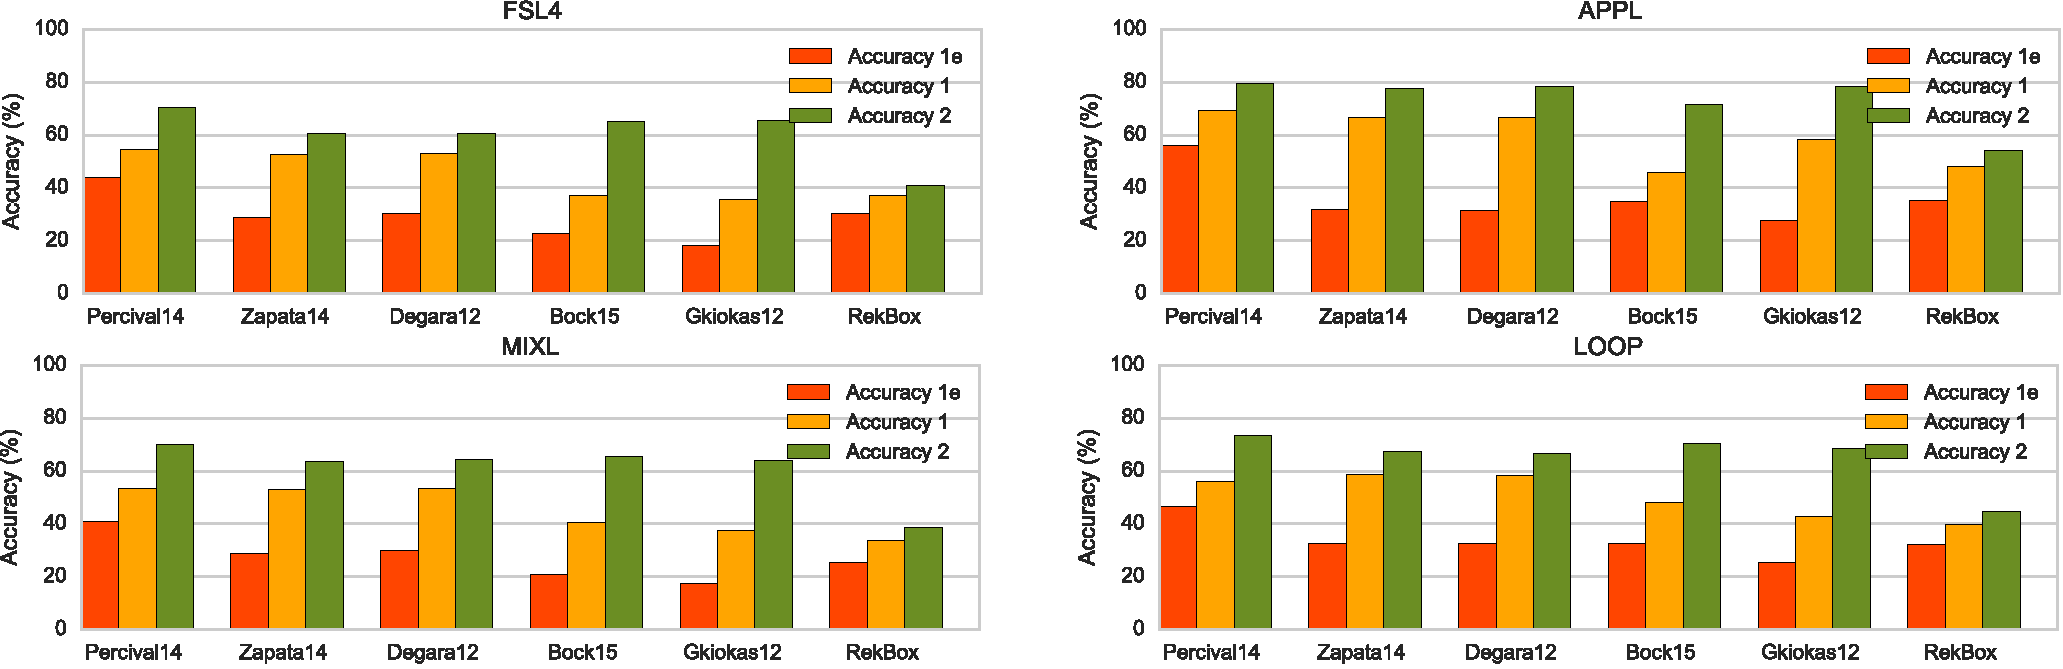
\includegraphics[width=0.95\textwidth]{figs/overall_accuracies-crop.pdf}}
 \caption{Overall accuracy for the six tempo estimation algorithms tested against the four datasets.}
 \label{fig:overall_accuracies}
\end{figure*}

In our evaluation we compare six existing tempo estimation algorithms.
These have been chosen based on their availability and to represent different approaches to the tempo estimation task.
We now briefly describe each of the algorithms, further details on how the algorithms work can be found in corresponding papers.

\begin{itemize}
	\item \textbf{Gkiokas12}: Gkiokas et. al.~\cite{Gkiokas2012} propose a tempo estimation algorithm based on the separation of the audio signal into its percussive and harmonic components. Periodicity analysis is carried out by convolving extracted features (filterbank energies for the percussive component and chroma features for the harmonic component) with a bank of resonators. Output tempo value is computed by applying heuristics based on metrical relations knowledge (meter, tactus, tatum) to the periodicity vector. We use a Matlab implementation of the algorithm kindly provided to us by the authors.
	\item \textbf{Degara12}: Degara et. al.~\cite{Degara2012} describe a probabilistic approach for beat tracking based on inter-onset-interval times and a salience measure for individual beat estimates. This method builds from previous probabilistic beat tracking methods such as Klapuri et. al.~\cite{Klapuri2006}. We use the implementation provided in Essentia, where final estimated tempo is given based on the mean of estimated beat intervals (see RhythmExtractor2013 algorithm\footnote{http://essentia.upf.edu/documentation/algorithms\_reference.html}).
	\item \textbf{Zapata14}: Zapata et. al.~\cite{Zapata2014} propose a beat tracking algorithm which estimates beat positions based on computing the agreement of alternative outputs of a single model for beat tracking using different sets of input features (i.e.,~using a number of onset detection functions based on different audio features). Again, we use the implementation provided in Essentia, which outputs a single BPM estimate based on estimated beat intervals.
	\item \textbf{Percival14}: Percival and Tzanetakis~\cite{Percival2014} describe a tempo estimation algorithm optimised for low computational complexity that combines several ideas from existing tempo estimation algorithms and simplifies their steps. The algorithm computes an onset strength function based on filtered spectral flux from which tempo lag candidates are estimated using autocorrelation. The most prominent tempo lag is selected and a simple decision tree algorithm is used to chose the octave of the final BPM output. We use a Python implementation of the algorithm provided by the authors in their original paper\footnote{http://opihi.cs.uvic.ca/tempo}.
	\item \textbf{B\"{o}ck15}: B\"{o}ck et. al.~\cite{Sebastian2015} propose a novel tempo estimation algorithm based on a recurrent neural network that learn an intermediate beat-level representation of the audio signal which is then feed to a bank of resonating comb filters to estimate the dominant tempo. This algorithm got the highest score in ISMIR 2015 Audio Tempo Estimation task. An implementation by the authors is included in the open-source Madmom audio signal processing library\footnote{http://github.com/CPJKU/madmom}.
	\item \textbf{RekBox}: We also include an algorithm from a commercial DJ software, Rekordbox\footnote{http://rekordbox.com}. Details on how the algorithm works are not revealed, but a freely downloadable application is provided that can analyse a music collection and export the results in a machine-readable format.
\end{itemize}


\subsection{Methodology}\label{sec:methodology}

%Similarly to previous tempo estimation works, we follow the methodology described by Gouyon et al.~\cite{Gouyon2006} to test the aforementioned algorithms against the four collected datasets. 
%We compute the two accuracy measures \emph{Accuracy 1} and \emph{Accuracy 2}.
%Accuracy 1 is the percentage of instances whose estimated BPM is within 4\% of the annotated ground truth.
%Accuracy 2 is the percentage of instances whose estimated BPM is within a 4\% of a multiple of $\frac{1}{3}$, $\frac{1}{2}$, 1, 2, or 3 times the ground truth BPM.
%In this way, Accuracy 2 also considers as good estimates those instances whose estimated tempo is either half, double, triple or one third of the annotated tempo, considering that tempo perception can be understood at different metrical levels~\cite{Gouyon2006}.
For testing the above algorithms against the four collected datasets we follow standard practice and adopt the methodology described by Gouyon et al.~\cite{Gouyon2006}.
In addition to the standard \emph{Accuracy 1} and \emph{Accuracy 2} measures\footnote{Accuracy 1 is the percentage of instances whose estimated BPM is within 4\% of the annotated ground truth. Accuracy 2 is the percentage of instances whose estimated BPM is within a 4\% of $\frac{1}{3}$, $\frac{1}{2}$, 1, 2, or 3 times the ground truth BPM.}, we add an extra measure that we call \emph{Accuracy 1e} and that represents the percentage of instances whose estimated BPM is exactly the same as the ground truth after rounding the estimated BPM to the nearest integer. Accuracy 1e is therefore more strict than Accuracy 1.
The reason why we added this extra accuracy measure is that, imagining a music creation context where loops can be queried in a database, it is of special relevance to get returned instances whose BPM exactly matches that specified as target. %It can still be argued that considering the time stretching capabilities of most music production environments, it is not strictly needed that returned algorithms have exactly the same tempo as these can be easily transformed. Nevertheless, we understand that the three accuracy measures together can give more informative results.

Besides the overall accuracy measurements, we are also interested in observing how accuracy varies according to the confidence values that we estimate (Sec.~\ref{sec:confidence_measure}).
We can intuitively imagine that if we remove instances from our datasets whose estimated BPM confidence is below a certain threshold, the overall accuracy results will increase. 
However, the higher we set the minimum confidence threshold, the smaller the size of filtered dataset will be.
Hence, we want to quantify the relation between the overall accuracy and the total number of music loops that remain in a dataset after filtering by minimum confidence.
To do that, given one of the aforementioned accuracy measures, we can define a minimum confidence threshold $\gamma$ and a function $A(\gamma)$ that represents overall BPM estimation accuracy when only evaluating loop instances whose estimated confidence value is above $\gamma$ for a given dataset and tempo estimation algorithm.
Similarly, we can define another function $N(\gamma)$ which returns the percentage of instances remaining in a dataset after filtering out those whose estimated confidence value (for a given tempo estimation method) is below $\gamma$. $A(\gamma)$ and $N(\gamma)$ can be understood as standard precision and recall curves, and therefore we can define a combined score measure $S(\gamma)$ doing the analogy with an f-measure computation:

$$ S(\gamma) = 2 \cdot \frac{A(\gamma) \cdot N(\gamma)}{A(\gamma) + N(\gamma)}.$$

An overall score for a given dataset, tempo estimation algorithm and accuracy measure can thus be given by taking the mean of $S(\gamma)$, $\bar S$.

\section{Results}\label{sec:results}

\subsection{Overall accuracy}\label{sec:results_overall}

Overall accuracy results show that Percival14 obtains the highest accuracy scores for all accuracy measures and all datasets except for the LOOP dataset, in which highest score for Accuracy 1 is obtained by Zapata14 (Fig.~\ref{fig:overall_accuracies}). Considering the data from all datasets at once, mean accuracy values for Percival14 range from 47\% (Accuracy 1e) to 73\% (Accuracy 2), with an average increase of 7\% accuracy when compared with the second best-scored method. With a few exceptions, pairwise accuracy differences between Percival14 and the second best-scored method in all datasets and accuracy measures are statistically significant using McNemar's test and a significance value of $\alpha=0.01$ (i.e.,~$p \ll 0.01$). 
We also observe that accuracies for the APPL dataset tend to be higher than for other datasets. This can be explained by the fact that APPL contains professionally created and curated loops, while the other datasets contain user contributed content, not necessarily created by professionals (Mixcraft's loop library also contains content gathered from online repositories).

\subsection{Accuracy vs confidence measure}\label{sec:results_confidence}

\begin{figure}
 \centerline{
 \includegraphics[width=0.91\columnwidth]{figs/accuracy_vs_confidence_FSL4-crop.pdf}}
 \caption{Accuracy vs confidence measure for FSL4 dataset. Lower bounds of the filled areas correspond to Accuracy 1e, while upper bounds correspond to Accuracy 2. Solid lines represent the number of instances remaining in the dataset.}
 \label{fig:accuracy_vs_confidence_FSL4}
\end{figure}

Fig.~\ref{fig:accuracy_vs_confidence_FSL4} shows the accuracy of the three best-scoring tempo estimation algorithms and the number of instances remaining in the dataset when filtering by different values of a confidence threshold $\gamma$ (Sec.~\ref{sec:methodology}).
%Equivalent plots for the other datasets can be found in the IPython notebook published in the aforementioned public source code repository.
As we expected, we can see how accuracy increases with $\gamma$ but the number of instances decreases.
Interestingly, we observe that the number of instances decays later for estimations performed with Percival14 algorithm than for the other algorithms.
This reflects the fact that Percival14 produces better BPM estimates.
Filtering by the confidence measure, a potential user searching for loops in a dataset could define a minimum threshold to get more accurate results at the expense of getting less loops returned. 
For instance, if we set a hard confidence threshold of $\gamma=0.95$ (vertical line in Fig.~\ref{fig:accuracy_vs_confidence_FSL4}), we find that the accuracies for Percival14 method range, on average, from 67\% (Accuracy 1e) to 92\% (Accuracy 2) while preserving an average of 52\% of the instances. 
Interestingly enough, we observe that when setting that hard threshold, reported RekBox accuracies outperform these of Percival14 in all datasets, with an average increase ranging from 2\% for Accuracy 2 to 14\% for Accuracy 1e (all statistically significant with $p \ll 0.01$). 
We attribute this to the fact that RekBox seems to have a built-in confidence measure thresholding step in which the algorithm outputs 0 BPM when the analysis does not meet certain confidence requirements. Therefore, once filtering the datasets by $\gamma$ (even with small values), all those instances whose BPM estimation is 0 BPM get discarded. Nevertheless, it is also important to note that filtering with the hard threshold, RekBox only preserves an average of 31\% of the instances (lower than the 52\% reported above by Percival14). %This, combined with the observed increase of Accuracy 1e, implies that the built-in confidence of RekBox tends to discard instances whose BPM estimation is a multiple of the ground truth BPM.

If we look at the combined accuracy and confidence measure $\bar S$ described in Sec.~\ref{sec:methodology}, we again find that Percival14 obtains the best score in all datasets and for all accuracy measures (i.e.~for $A(\gamma)$ computed with Accuracy 1e, Accuracy 1 or Accuracy 2). This means that Percival14 offers the overall best balance between estimation accuracy and number of preserved instances in the dataset when filtering by a minimum confidence threshold. %Hence, and following the previous example of a user searching for loops, Percival14 seems to be the best method to use for maximising both accuracy and number of results.


\subsection{Comparison of confidence measures}

\begin{figure}
 \centerline{
 \includegraphics[width=0.91\columnwidth]{figs/confidence_ffont_vs_confidence_zapata_FSL4-crop.pdf}}
 \caption{Comparison of our proposed confidence measure with the confidence measure proposed in~\cite{Zapata2012} for FSL4 dataset and Zapata14 tempo estimation algorithm.}
 \label{fig:confidence_vs_zapata_confidence_FSL4}
\end{figure}

Zapata et. al.~\cite{Zapata2012} propose a confidence measure that can be used for tempo estimation and that is based on computing the mutual agreement between an ensemble of tempo estimation algorithms. % that take different sets of input features.
To make this confidence measure numerically comparable to the one we propose, we normalise the confidence output of Zapata et. al. to take values from 0 to 1.
Similarly to Fig.~\ref{fig:accuracy_vs_confidence_FSL4}, we plot the estimation accuracy and the number of remaining instances as a function of a minimum confidence threshold $\gamma$ (Fig.~\ref{fig:confidence_vs_zapata_confidence_FSL4}). 
We observe that Zapata's confidence measure allows to achieve accuracies which are around 15\% higher than when using our confidence. However, the number of remaining instances in the dataset is drastically reduced, and accuracy values for $\gamma > 0.75$ become inconsistent. 
Looking at the $\bar S$ score, we find that Zapata14 in combination with our confidence measure gets better results than when using the original measure, with an average $\bar S$ increase of 17\%, 29\% and 31\% (for the three accuracy measures respectively). 
This indicates that our confidence measure is able to better maximise accuracy and number of remaining instances.


\section{Conclusion}\label{sec:conclusion}
In this paper paper we have compared several tempo estimation algorithms using four datasets of music loops.
We also described a simple confidence measure for tempo estimation algorithms and proposed a methodology for evaluating the relation between estimation accuracy and confidence measure. 
This methodology can also be applied to other MIR tasks, and we believe it encourages future research to put more emphasis on confidence measures.
We found that by setting a high enough minimum confidence threshold, we can obtain reasonably high tempo estimation accuracies while preserving half of the instances in a dataset. 
However, these results are still far from being optimal: if we only consider exact BPM estimations (Accuracy 1e), the maximum accuracies we obtain are still generally lower than 70\%.
We foresee two complementary ways of improving these results by \emph{i)} adapting tempo estimation algorithms to the case of music loops (e.g.~taking better advantage of tempo steadiness and expected signal duration), and \emph{ii)} developing more advanced confidence measures that take into account other properties of loops such as the beat strength or the rate of onsets.
Overall, the work we present here contributes to the improvement of the reusability of unstructured music loop repositories.

\section{Acknowledgments} 
This work has received funding from the European Union's Horizon 2020 research and innovation programme under grant agreement No 688382.

\bibliography{biblio}
\end{document}
